\section{星云资产监管方案}

如图~\ref{fig:assets},星云资产包括社区公共资产和星云基金会监管资产两部分。

\subsection{社区公共资产}

\subsubsection{构成}

\begin{itemize}
	\item 星云非技术白皮书资产分配相关章节中提及的社区生态预留部分:35,000,000 NAS(35\%)
    \item 共识记账系统增发,每日自动产生( 8,219.1744 NAS/日),包括:
	    \begin{itemize}
			\item 2\%:共识记账收入 (截止节点分发之前)
			\item 1\%:星云理事会项目发展资金储备
		\end{itemize}
	\item 开发者激励协议(Developer Incentive Protocol,DIP)~\cite{mauvepaper}产生的原生激励: 自2019年5月13日起产生,初始为1\%
\end{itemize}

\subsubsection{管理}

公共资产属于社区,通过星云链上治理流程由社区共同参与管理,星云理事会负责监督。

\subsection{星云基金会资产}

\subsubsection{构成}

\begin{itemize}
	\item 星云非技术白皮书资产分配相关章节中提及的星云团队预留部分:20,000,000 NAS(20\%)
    \item 星云社区发展基金(生态投资余额):5,000,000 NAS(5\%)
	\item 早期私募所得项目发展资金
	\item 早期生态投资所得
\end{itemize}

\subsubsection{管理}

星云基金会资产由星云基金会管理,星云基金会应确保资产整体使用情况公开透明。

\begin{figure}
	\centering
	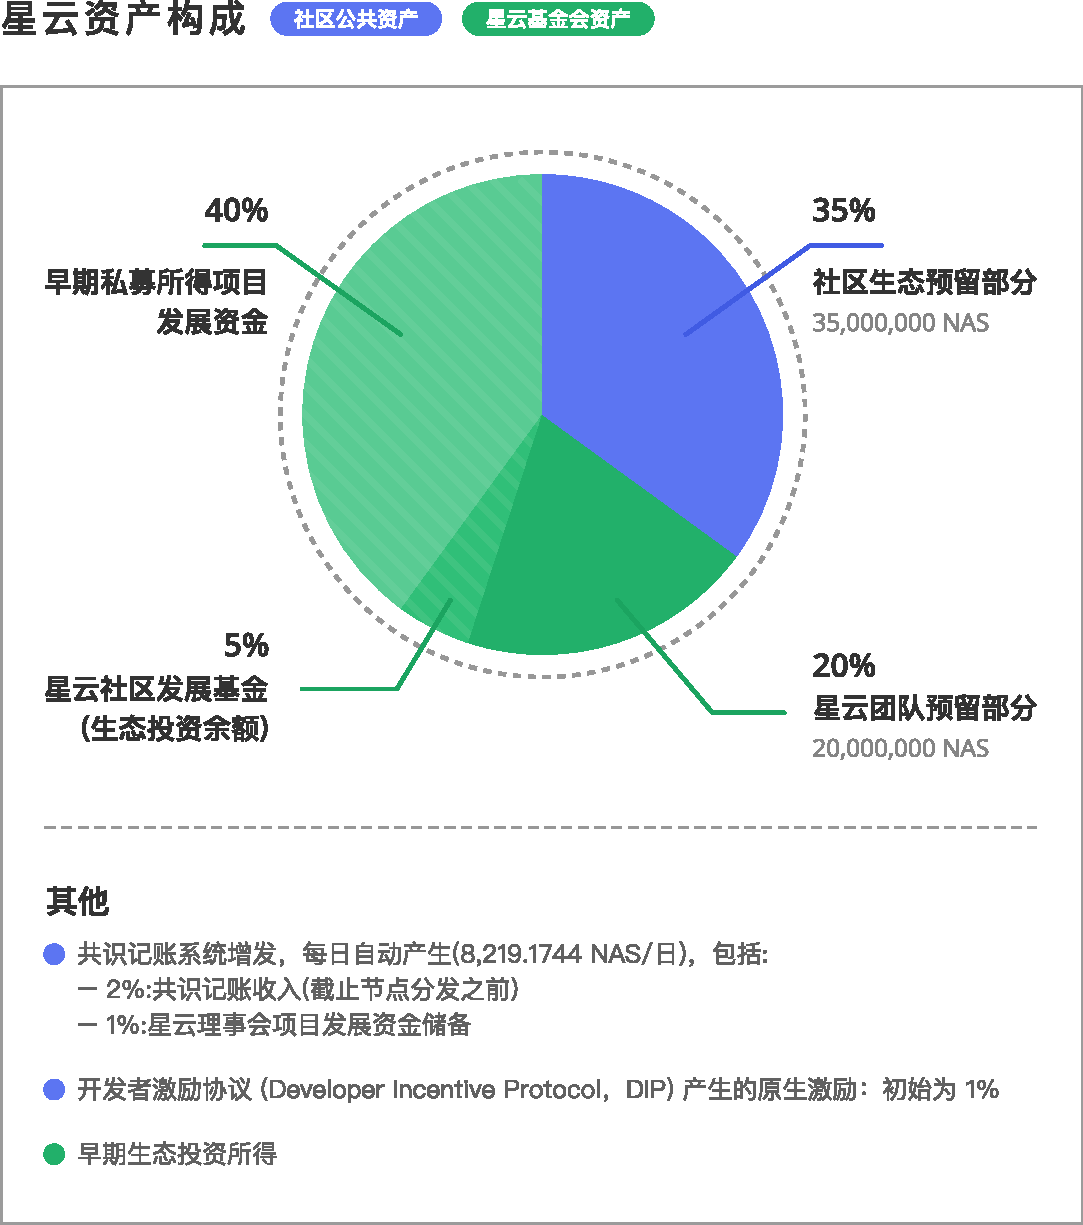
\includegraphics[width=1\textwidth]{../common/ch/assets.pdf}
	\caption{星云资产构成 \label{fig:assets}}
\end{figure}